\documentclass[12pt,a4paper]{article}
\usepackage[T1]{fontenc}
\usepackage[utf8]{inputenc}
\usepackage{lmodern}
\usepackage[margin=2.5cm]{geometry}
\usepackage{amsmath,amssymb,graphicx,booktabs,array,placeins}
\usepackage[hidelinks]{hyperref}
\graphicspath{{../figures/separable/}}
\title{When does logistic regression converge?\\[0.4em]\large Loss, parameter growth, and stopping criteria on separable data}
\author{Mohamed Aziz Mrad}
\date{22 November 2026}
\begin{document}
\maketitle
\section{Introduction and research question}
\subsection{Starting question}
After implementing and comparing optimization methods for logistic regression, I studied support vector machines and maximum-margin geometry through Stanford CS229 lectures. This prompted me to investigate how logistic gradient descent selects a separating boundary on separable data. In particular, I wanted to understand whether decreasing loss implies convergence to a finite parameter vector, and how the resulting direction relates to the maximum-margin separator.

To connect these questions with the research literature, I discussed them with AI, which suggested Soudry et al. as a relevant reference. The paper provided a precise theoretical question: whether the direction selected by logistic gradient descent approaches the maximum-margin direction even as the parameter norm grows.

To complement this resource with academic advice and connect the project with my coursework, I subsequently contacted my topology instructor. He suggested examining conditions under which minimizing sequences are bounded, and their connections with coercivity, compactness, and the existence of a minimum. This provided a complementary mathematical framework: a bounded minimizing sequence for a continuous function on a finite-dimensional space has a convergent subsequence whose limit attains the infimum. For separable logistic regression, the infimum is zero but is not attained at any finite parameter, so a minimizing sequence cannot remain bounded.

\subsection{Objective and quantities that must be distinguished}
The labels are -1 and +1. X stores observations as rows. All models here are homogeneous: the score is $x_i^\top w$, with no intercept. The mean logistic loss has no explicit regularization penalty.

\[
L(w)=\frac{1}{n}\sum_{i=1}^{n}\log(1+e^{-y_i x_i^T w}),\qquad w_{t+1}=w_t-\alpha\nabla L(w_t)
\]
Loss convergence, parameter convergence, and convergence of normalized direction are different questions. For nonzero w, define u=w/$\|w\|$, directional error e=$\|u-u_{\mathrm{SVM}}\|$, and signed geometric margin $\gamma=\min_i y_i x_i^\top w/\|w\|$. A positive margin is the closest-point distance when every observation is correctly classified. A negative margin records misclassification. Direction and margin are undefined at zero weights.

\subsection{Why a minimizing sequence can escape to infinity}
If v strictly separates the finite dataset, every $y_i x_i^\top v$ is positive. Hence $L(cv)$ tends to zero as c tends to infinity, while every finite w has $L(w)>0$. The infimum is zero but is not attained. Any bounded subsequence of a minimizing sequence would have a convergent further subsequence in finite dimensions; continuity would make its limit attain zero, a contradiction. Thus every minimizing sequence must eventually leave every bounded ball.

\subsection{Published asymptotic result and scope}
Under the separability, smoothness, exponential-tail and sufficiently small fixed-step assumptions in Soudry et al. [1, Lemma 1 and Theorem 3], logistic gradient descent has loss tending to zero, diverging parameter norm, and normalized direction approaching the normalized homogeneous hard-margin SVM solution. These are cited theoretical conclusions, not proved by the finite experiments below. The experiment does not test the paper's multiclass or neural-network extensions.

\FloatBarrier
\section{Experimental design and numerical checks}
\subsection{Reference problem and learning rates}
\[
\widehat w=\arg\min_w\frac{1}{2}\|w\|^2\quad\mathrm{subject\ to}\quad y_i x_i^T w\geq1\quad\forall i
\]
Gurobi solves this convex quadratic program without an intercept. At its optimum the smallest functional margin is 1, giving maximum geometric margin $1/\|\widehat{w}\|$. The constructing separator is not substituted for this numerical reference.

For the mean logistic loss, the Hessian is $X^\top D X/n$, where D has diagonal entries between 0 and 1/4. Thus $B=\|X\|_2^2/(4n)$ bounds its largest eigenvalue. Translating the paper's summed-loss convention gives the sufficient condition $0<\alpha<2/B$. The suite uses $\alpha$=c/B for c in $\{$0.1,0.5,1$\}$; all are within that bound. B denotes the matrix spectral-norm bound, not an elementwise bound.

\subsection{Datasets and budgets}
\begin{center}
\small
\begin{tabular}{@{}p{0.221\textwidth}p{0.699\textwidth}@{}}
\toprule
\textbf{Dataset} & \textbf{Construction} \\
\midrule
Four points & (1,0), (-1,0), (2,1), (-2,-1); labels +,-,+,- \\
Original random & 100 standard Gaussian 2D draws; y=sign(x1); discard x1=0 \\
Added clearance & Same points/labels; replace x1 by y*(abs(x1)+0.3) \\
\bottomrule
\end{tabular}
\end{center}
The random seeds are 42, 0 and 1. All retained samples have 100 observations and both classes. The suite comprises seven datasets times three step choices: 21 runs, each initialized at zero and capped at 100,000 updates. The paired clearance experiment changes geometry, B, and the SVM reference; it is not a pure isolation of margin. The original exploratory run uses $\alpha$=0.1 and is kept separate from suite results.

\subsection{Checks actually executed}
Central finite differences at w=(0.3,-0.2), h=1e-5, agreed with the analytical gradient on every dataset; the largest absolute discrepancy was below 1e-11. These are spot checks, not proofs for every input. Gurobi reported an optimum for each reference. Checks tested feasibility, nonnegative dual multipliers, stationarity $w=A^\top\lambda$, complementary slackness, and primal-dual objective agreement, with $A=\operatorname{diag}(y)X$. All configured numerical tolerances passed; the largest recorded relative objective gap was below 6e-11.

Every iterate was checked for finite values; no loss increase greater than 1e-12 was recorded. Stopping thresholds 1e-2, 1e-3, 1e-4 and 1e-5 were checked at every iterate. A first threshold crossing was recorded without terminating the shared trajectory. Unmet thresholds are explicitly marked as iteration-budget stops. Log-spaced trajectory samples, exact datasets, reference checks and settings are saved.

\FloatBarrier
\section{Does a small loss imply an accurate direction?}
The four-point case has an exact reference: its first pair forces $w_1\geq 1$, so the smallest possible norm is 1. The vector (1,0) attains it and satisfies all four constraints, with signed scores (1,1,2,2). Gurobi agrees within numerical precision. Starting at zero does not initially separate the classes.

\begin{figure}[htbp]
\centering
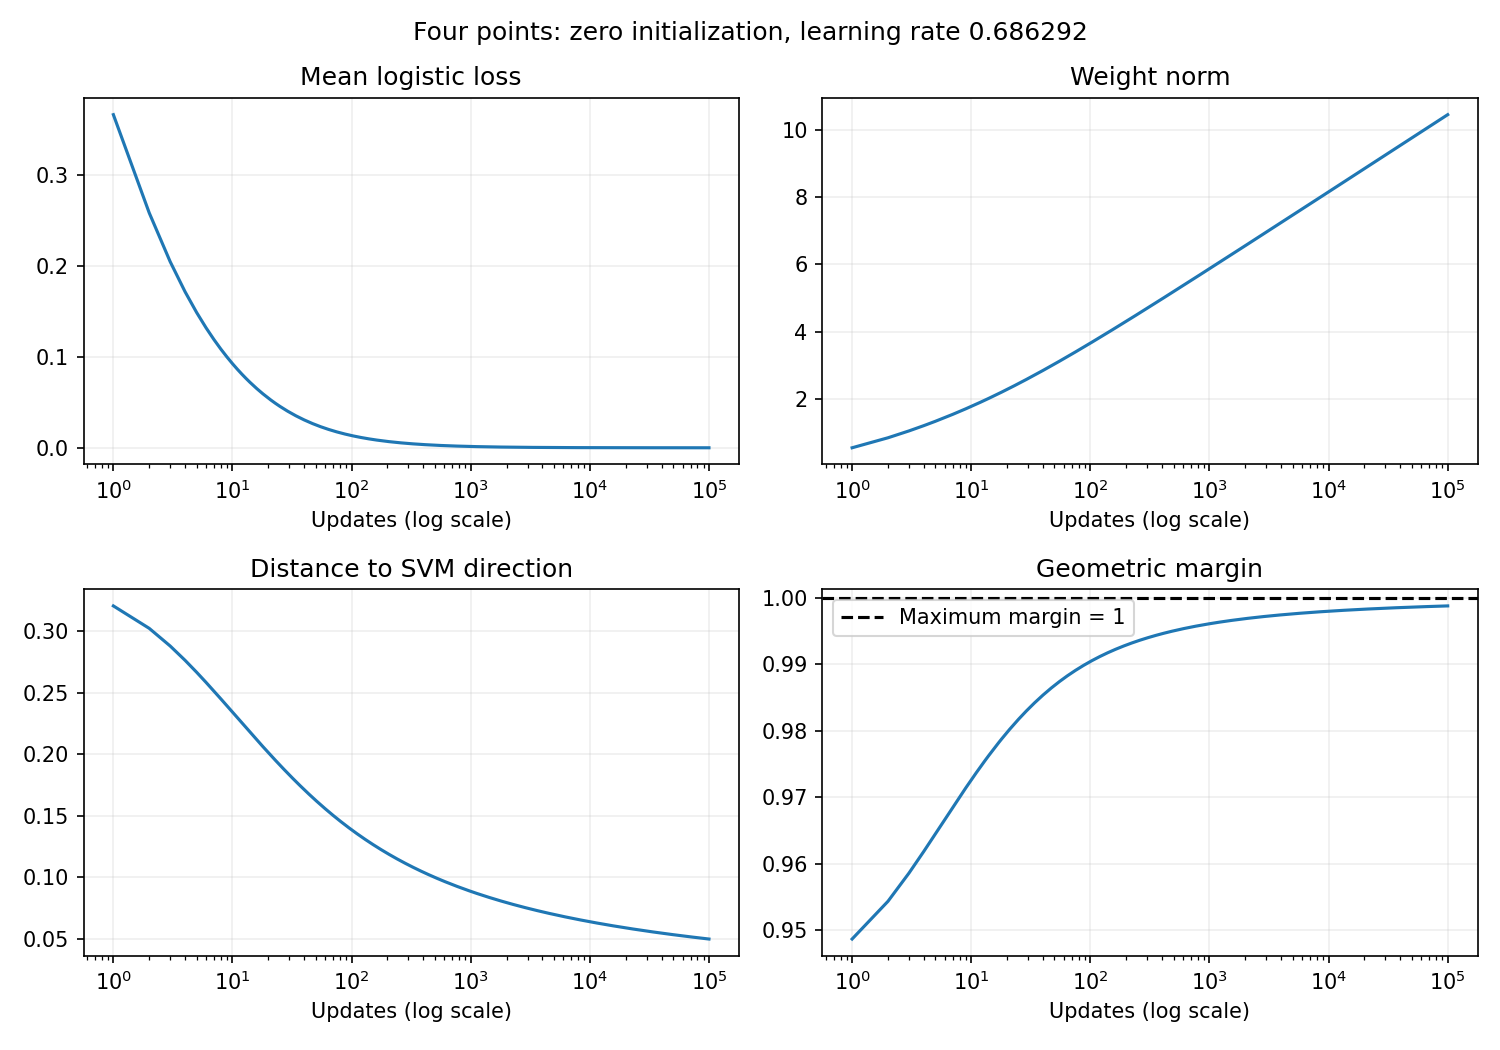
\includegraphics[width=\textwidth]{review_01_four_points.png}
\caption{Four-point control: loss, weight norm, directional error and geometric margin.}
\end{figure}
\begin{center}
\small
\begin{tabular}{@{}p{0.23\textwidth}p{0.23\textwidth}p{0.23\textwidth}p{0.23\textwidth}@{}}
\toprule
\textbf{Updates} & \textbf{Loss} & \textbf{Directional error} & \textbf{Geometric margin} \\
\midrule
1000 & 0.001440972 & 0.08861 & 0.99607 \\
10000 & 0.0001455126 & 0.06394 & 0.99796 \\
100000 & 1.456873e-05 & 0.04989 & 0.99876 \\
\bottomrule
\end{tabular}
\end{center}
Zero initialization and $\alpha$=0.5/B, approximately 0.686292. Horizontal axes are logarithmic. Directional error decreased at every checked update in this particular run. From 1,000 to 10,000 updates, loss falls by about a factor of ten, while directional error falls by only about 28\%. The finite observations support slow directional progress relative to loss improvement; they do not estimate or prove an asymptotic rate.

\FloatBarrier
\section{Does a larger safe learning rate always help?}
The first extension was to vary the step size while holding each dataset fixed. Within a panel, the same numerical B is used for all three choices. Across panels, equal c/B rules correspond to different absolute learning rates.

\begin{figure}[htbp]
\centering
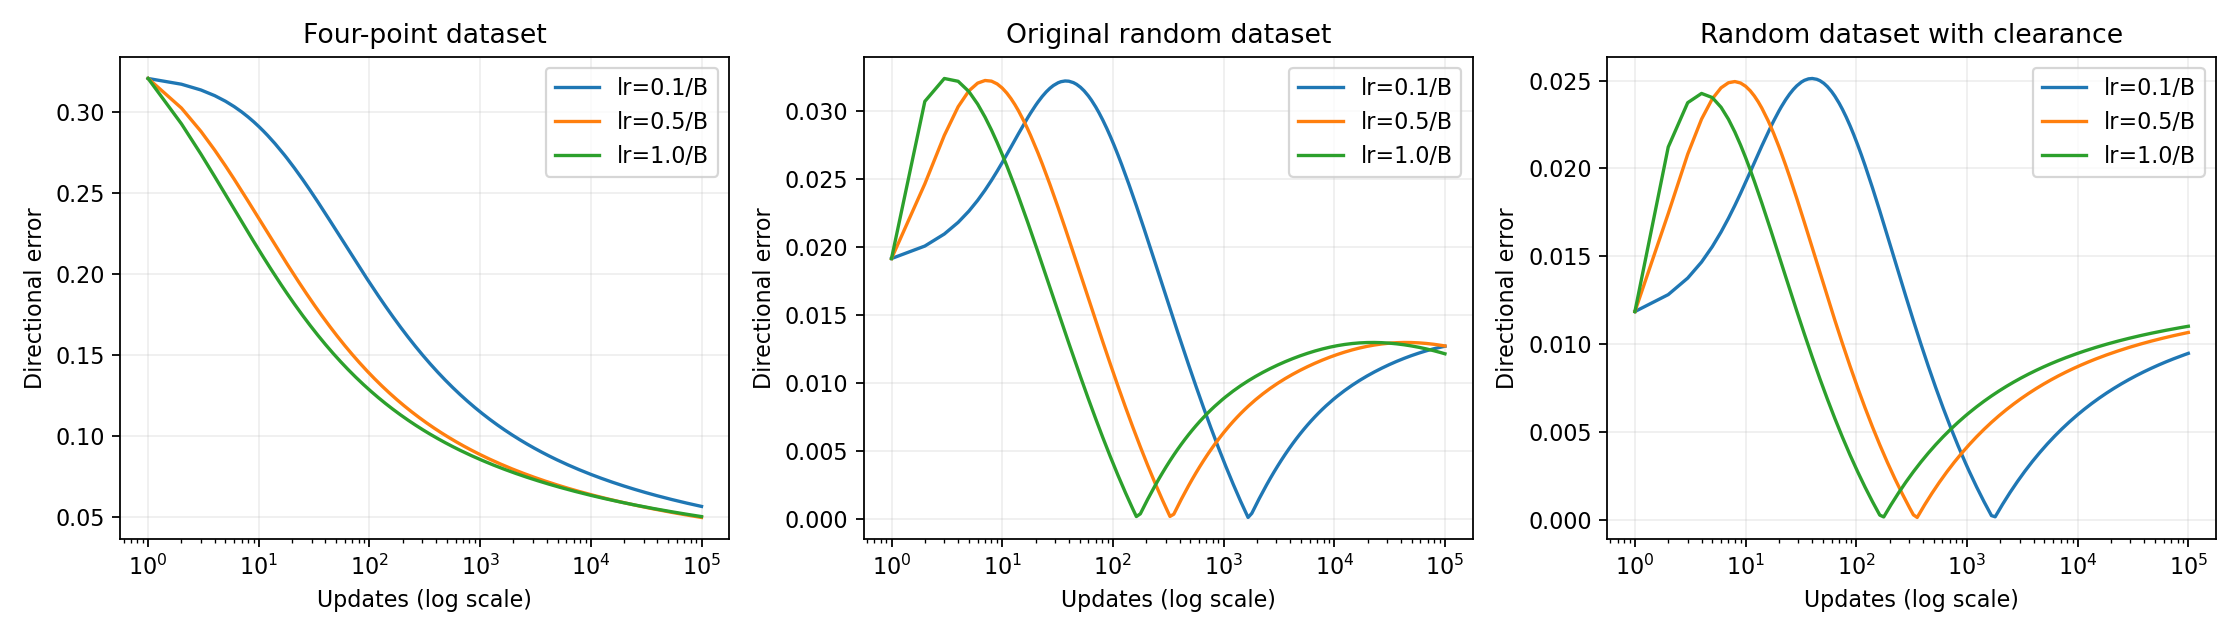
\includegraphics[width=\textwidth]{step_size_comparison.png}
\caption{Directional error for three safe step sizes, with random seed 42.}
\end{figure}
\begin{center}
\small
\begin{tabular}{@{}p{0.23\textwidth}p{0.23\textwidth}p{0.23\textwidth}p{0.23\textwidth}@{}}
\toprule
\textbf{Dataset} & \textbf{c=0.1} & \textbf{c=0.5} & \textbf{c=1.0} \\
\midrule
Four points & 0.05669 & 0.04989 & 0.05042 \\
Original random & 0.01272 & 0.01275 & 0.01217 \\
Added clearance & 0.00947 & 0.01066 & 0.01101 \\
\bottomrule
\end{tabular}
\end{center}
Directional error versus update count, and error at 100,000 updates. In the random cases, larger steps pass near the reference earlier, but the errors subsequently rise during part of the recorded interval. The largest step is not consistently best at the final budget; even for the four-point case, the medium step slightly outperforms the largest one at that endpoint.

\subsection{Answer and limitation}
A step-size condition ensuring loss descent does not ensure monotone directional improvement. Which step looks best depends on dataset and observation time. A passage near zero followed by a rise does not establish asymptotic divergence and does not contradict the cited directional limit. Increasing the budget indefinitely was not treated as a substitute for checking the implementation.

\FloatBarrier
\section{Are these observations specific to one random sample?}
Changing the seed tests sample-to-sample sensitivity. The learning-rate rule remains $\alpha$=0.5/B, although the actual rate changes with each sample. Each run is compared with its own independently solved SVM direction.

\begin{figure}[htbp]
\centering
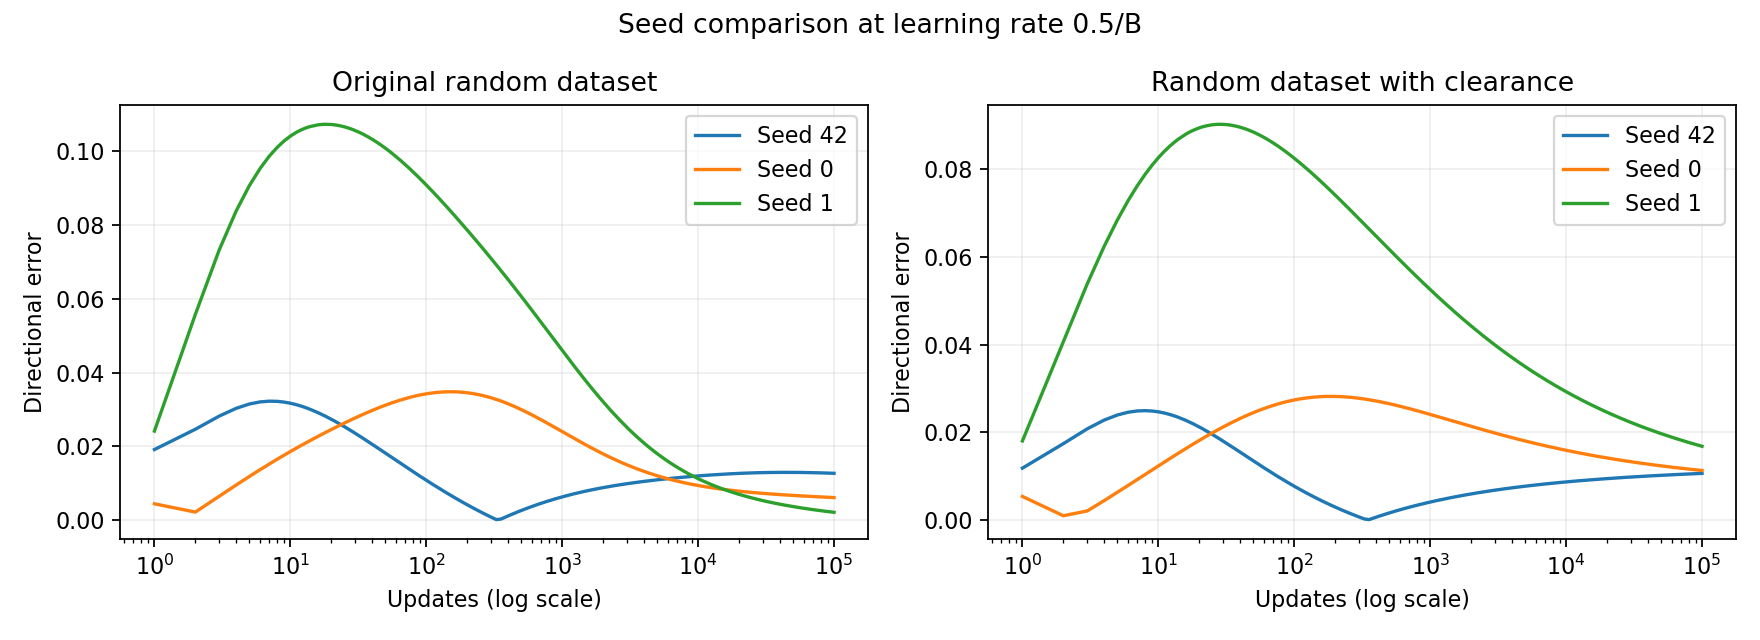
\includegraphics[width=\textwidth]{seed_comparison.png}
\caption{Directional error across three random seeds, using the rule alpha = 0.5/B.}
\end{figure}
\begin{center}
\small
\begin{tabular}{@{}p{0.307\textwidth}p{0.307\textwidth}p{0.307\textwidth}@{}}
\toprule
\textbf{Seed} & \textbf{Original final error} & \textbf{Added-clearance final error} \\
\midrule
42 & 0.01275 & 0.01066 \\
0 & 0.00618 & 0.01132 \\
1 & 0.00220 & 0.01683 \\
\bottomrule
\end{tabular}
\end{center}
Seed 1 has the largest early peak in the original family but the smallest final error. Rankings depend on the iteration budget. Added clearance lowers the observed peak for these three samples, yet increases the final error for seeds 0 and 1. The peak observation is descriptive, not a universal guarantee.

\subsection{Answer and limitation}
Neither an early error ranking nor greater clearance from the constructing separator reliably predicts the smallest final directional error in this comparison. The clearance modification also changes the optimal separator and numerical learning rate. Three seeds are a modest robustness check, not a statistical characterization of Gaussian samples.

\FloatBarrier
\section{What does the stopping criterion actually establish?}
The original question concerns stopping when $\|\nabla L\|<$ tolerance. A successful threshold stop reports a small gradient at the returned weights. It is not a certificate of parameter convergence, directional accuracy, or existence of a finite minimizer.

\begin{figure}[htbp]
\centering
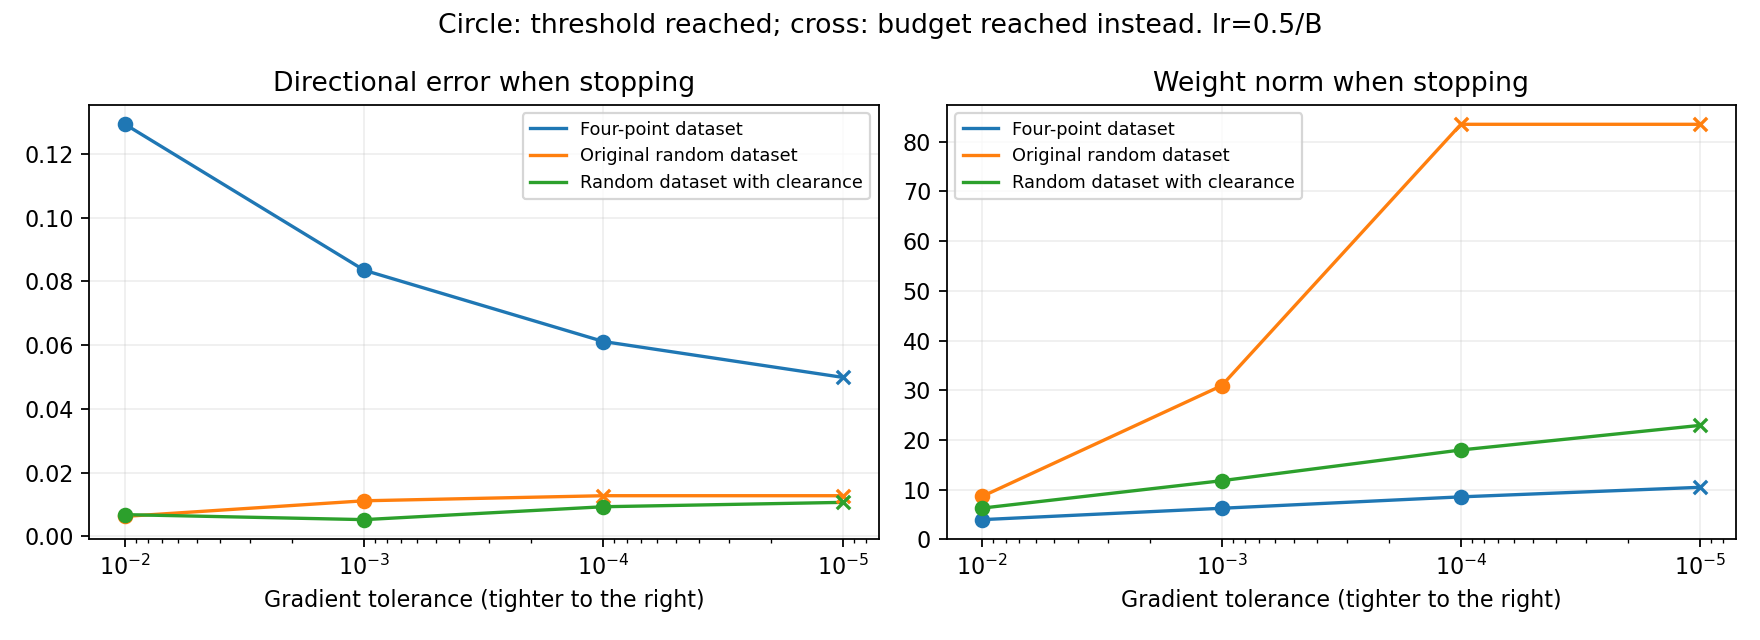
\includegraphics[width=\textwidth]{stopping_comparison.png}
\caption{Stopping tolerances: circles denote threshold crossings; crosses denote budget stops.}
\end{figure}
\begin{center}
\small
\begin{tabular}{@{}p{0.23\textwidth}p{0.23\textwidth}p{0.23\textwidth}p{0.23\textwidth}@{}}
\toprule
\textbf{Tolerance} & \textbf{Updates} & \textbf{Stop reason} & \textbf{Directional error} \\
\midrule
0.01 & 160 & Tolerance & 0.00626 \\
0.001 & 5505 & Tolerance & 0.01115 \\
0.0001 & 100000 & Budget & 0.01275 \\
1e-05 & 100000 & Budget & 0.01275 \\
\bottomrule
\end{tabular}
\end{center}
Seed 42 for random cases; $\alpha$=0.5/B. Circles mark actual threshold crossings; crosses mark budget stops. Connected crosses at different requested tolerances can represent the same iterate, not distinct converged solutions. The four-point final cross likewise did not satisfy its requested tolerance.

\subsection{Answer}
On the original random dataset, tightening tolerance from 1e-2 to 1e-3 requires 160 versus 5,505 updates and returns a larger directional error, 0.00626 versus 0.01115. Both thresholds were actually reached. Neither 1e-4 nor 1e-5 is reached within the budget; their equal outputs are therefore expected. The growing returned norms are consistent with objective progress without finite parameter convergence. A finite tolerance has no dataset-independent directional-accuracy meaning in these experiments.

\FloatBarrier
\section{Could the support-vector selection be a tolerance artifact?}
The unexpected directional trajectory prompted a separate numerical question: would changing the np.isclose tolerance change which observations were called support vectors? This question arose during the student's inspection of the support-point plot. The test concerns the SVM reference, not a redefinition of the training labels.

\begin{figure}[htbp]
\centering
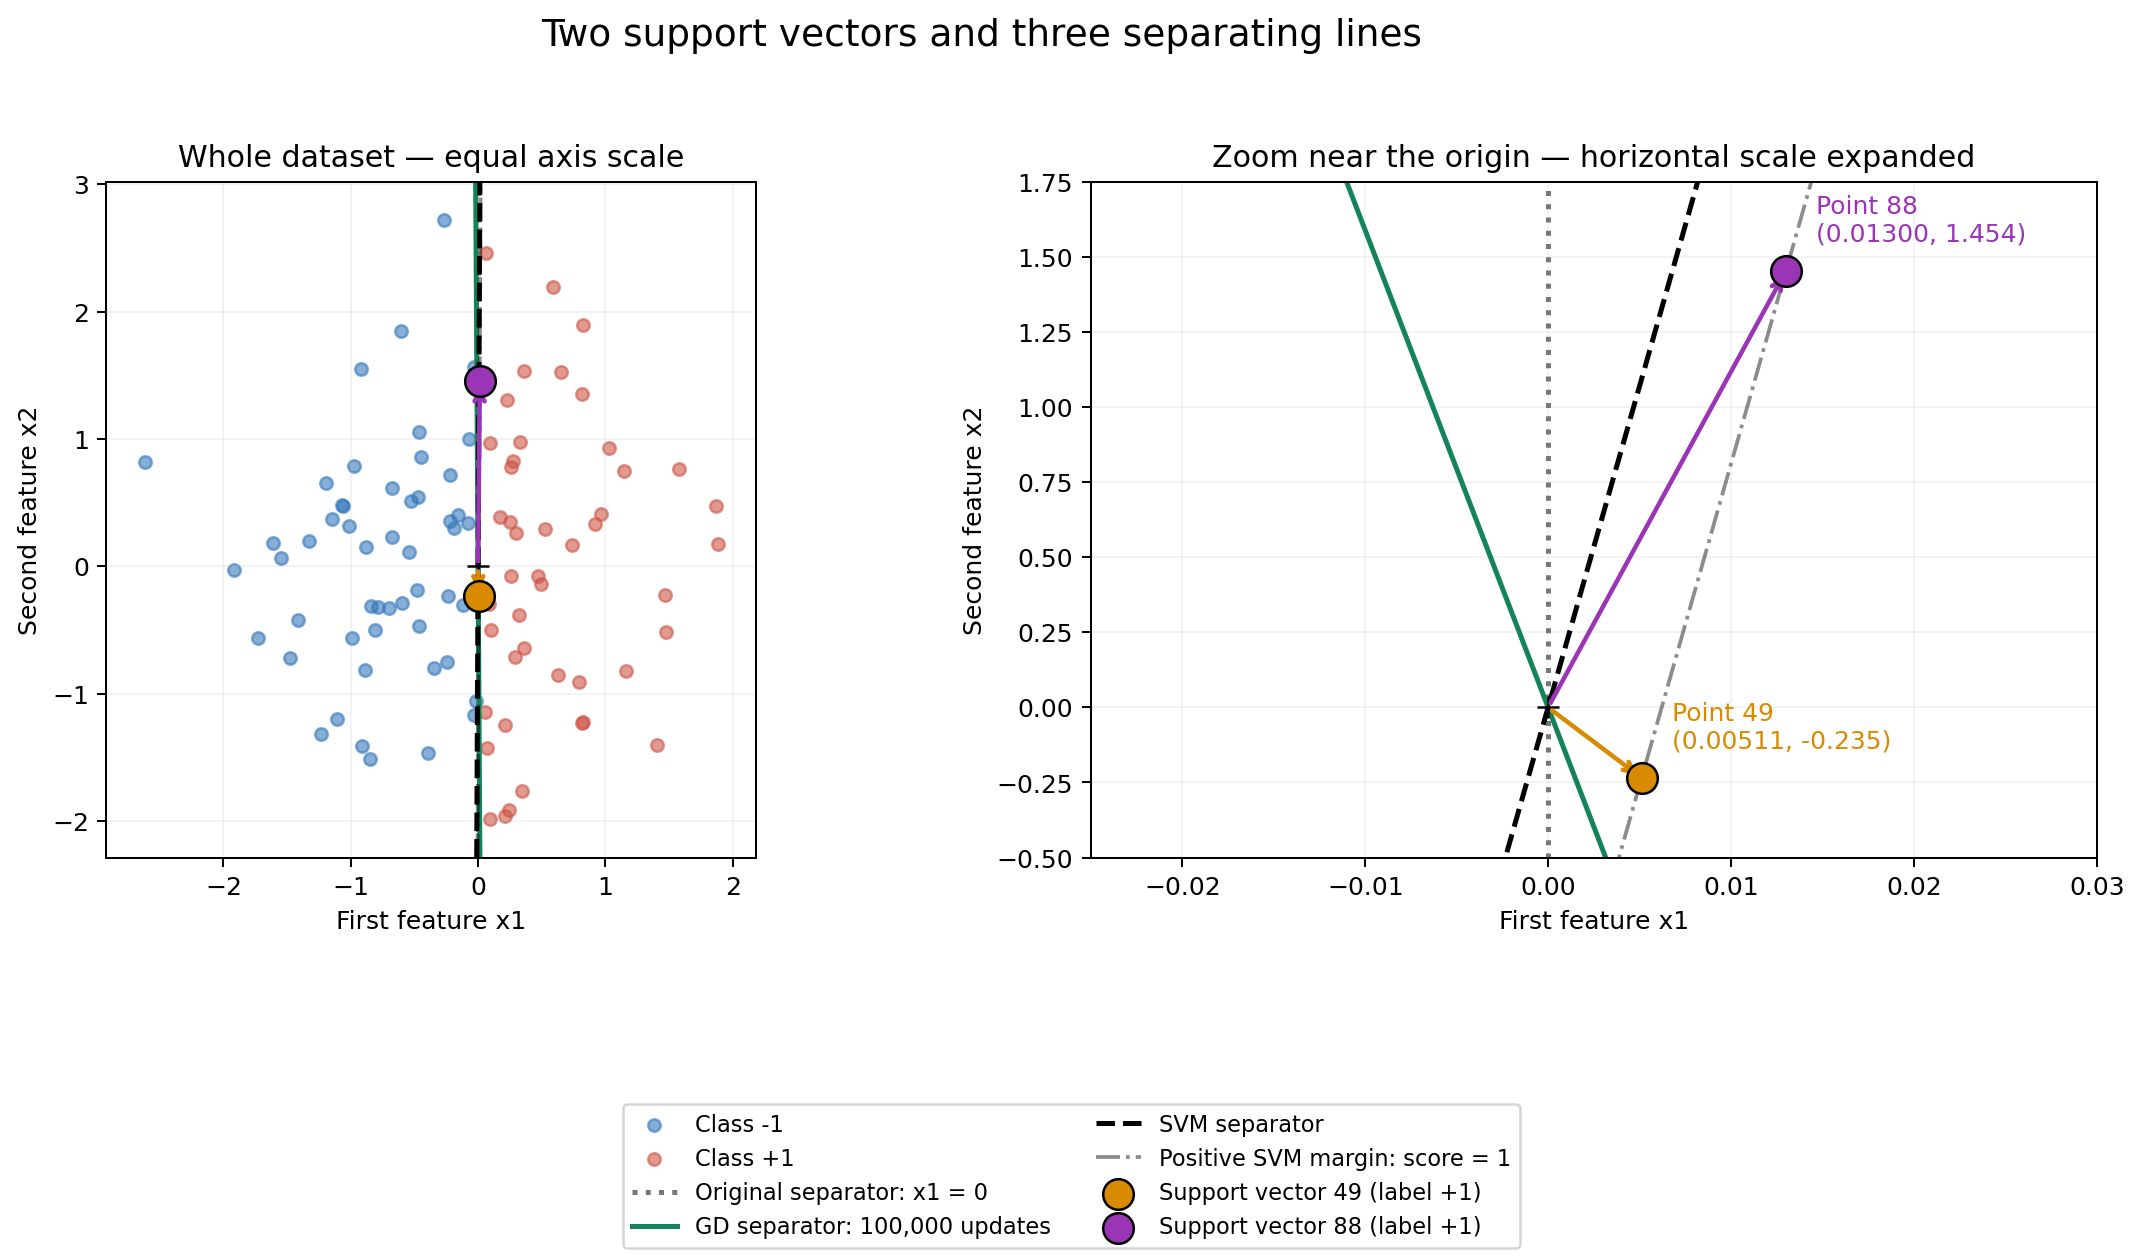
\includegraphics[width=\textwidth]{separators_support_vectors.png}
\caption{Constructing, gradient-descent and SVM separators, with the two support points highlighted.}
\end{figure}
Original seed-42 dataset, exploratory $\alpha$=0.1 run. Gray dotted: constructing separator. Green: gradient-descent separator after 100,000 updates. Black dashed: SVM separator. The two highlighted observations lie on the positive SVM margin boundary, not on the separator. Arrows are their position vectors, not gradient vectors. The zoom stretches the horizontal axis; angles and distances must not be read from its visual aspect ratio.

Indices 49 and 88 were selected at every tested absolute tolerance from 1e-4 to 1e-14 (relative tolerance zero). Their score residuals from 1 were 0 and approximately 6.66e-16; both solver multipliers were positive. The smallest score outside the selection was 1.37763. Thus the two selected constraints are supported as active within numerical precision, rather than being artifacts of the chosen 1e-6 threshold. Both have positive labels, which is possible because the no-intercept separator is constrained to pass through the origin.

\FloatBarrier
\section{Which observations drive the current update?}
The next diagnostic asked whether SVM support points necessarily turn a finite-time logistic update toward the SVM direction. For the exploratory seed-42 run at 100,000 updates, w=(29.75890453,0.18732167). The minimum signed score is about 0.10823 and its geometric margin about 0.003637, below the SVM maximum 0.006210. These scores use the final weights, not the original constructing separator.

\[
g_i=-\frac{1}{n}y_i x_i\,\sigma(-y_i x_i^T w),\qquad \nabla L(w)=\sum_i g_i
\]
The individual contributions were grouped by the SVM support mask. Their sum was checked against the implemented full gradient. The support group and other group were approximately (-0.00006851,-0.00384585) and (-0.00100167,+0.00383373). Their second components nearly cancel. Ranking individual contribution norms alone would miss this cancellation.

\begin{center}
\small
\begin{tabular}{@{}p{0.644\textwidth}p{0.276\textwidth}@{}}
\toprule
\textbf{Hypothetical update from the same w} & \textbf{Directional error} \\
\midrule
No update & 0.01096737852 \\
Support group only, step 0.1 & 0.01098029972 \\
Other group only, step 0.1 & 0.01095447544 \\
Combined gradient, step 0.1 & 0.01096739661 \\
\bottomrule
\end{tabular}
\end{center}
Contrary to the initial hypothesis, at this iterate the support-only step increases directional error, while the other-only step decreases it. Their combination slightly increases it. Point 88 has positive label and positive second feature: increasing $w_2$ improves its individual score and lowers its loss. SVM support status does not force every finite-time logistic update to align toward the SVM reference.

\subsection{What this diagnosis does and does not establish}
This is a local decomposition at fixed weights. The group steps are diagnostic evaluations, not independently trained models. They explain the direction of one update but neither prove the cause of the entire non-monotone interval nor predict when the trajectory will reverse. Non-support contributions are not ignored in the actual algorithm. The experiment does not establish the onset of the asymptotic regime.

\subsection{Main limitations}
All data are small, synthetic and two-dimensional. Budgets are finite; no asymptotic rate is fitted or established experimentally. The study tests three seeds and three safe step fractions, not a comprehensive distribution of configurations. No claims are made about validation performance, real-data generalization, Newton directional bias, regularization paths, multiclass models, or deep networks.

\FloatBarrier
\section{Conclusions and reproduction}
\subsection{Conclusions supported by this study}
The project distinguishes objective convergence, parameter growth, directional progress, and termination. The controlled four-point case exhibits a decreasing loss, growing norm, and improving direction and margin over the recorded run. Random samples reveal temporary reversals in directional error. Tighter gradient tolerances can return worse directional accuracy, while budget stops must be distinguished from satisfied tolerances. The numerical checks support the implementation and references; the asymptotic directional limit remains a theoretical input from [1].

\subsection{Reproduction}
Run commands from the numerical-optimization-ml repository root, using an environment containing NumPy, Matplotlib and gurobipy with a working Gurobi license. The saved configuration records Python 3.13.5, NumPy 2.1.3, Matplotlib 3.10.0 and Gurobi 14.0.0. Different versions and platforms can affect final floating-point digits.

\begin{center}
\small
\begin{tabular}{@{}p{0.515\textwidth}p{0.405\textwidth}@{}}
\toprule
\textbf{Command} & \textbf{Purpose} \\
\midrule
python -m experiments.separable$\_$diagnostics & Original seed-42 trajectory, support checks and local diagnostics \\
python -m experiments.separable$\_$control & Exact four-point control, $\alpha$=0.1 \\
python -m experiments.separable & 21-run suite, $\alpha$ in $\{$0.1,0.5,1$\}$/B \\
\bottomrule
\end{tabular}
\end{center}
The integrated suite saves data under results/separable/ and figures under figures/separable/, relative to the repository root. final$\_$results.csv contains one endpoint per run; stopping$\_$comparison.csv contains 84 threshold/budget endpoints; trajectory$\_$samples.csv contains sampled histories; reference$\_$checks.csv contains dataset and solver checks; data$\_$*.npz stores actual datasets and references; configuration.json records settings. Plots display selected seeds and step choices, while CSVs retain all runs. review$\_$01$\_$four$\_$points.png uses the suite rate 0.5/B, not the standalone control's rate 0.1.

\subsection{Reference}
[1] D. Soudry, E. Hoffer, M. S. Nacson, S. Gunasekar and N. Srebro. The Implicit Bias of Gradient Descent on Separable Data. Journal of Machine Learning Research 19(70), 1-57, 2018. Lemma 1 and Theorem 3. https://www.jmlr.org/papers/v19/18-188.html

\subsection{Acknowledgments}
This project was undertaken outside formal coursework. AI was used as a supplementary learning aid for unfamiliar concepts, individual questions, discussion of experimental behavior, and implementation support.

\FloatBarrier
\end{document}
